\documentclass{article}
\usepackage[utf8]{inputenc}
\usepackage[T1]{fontenc}
\usepackage{geometry}
\usepackage{enumitem}
\usepackage{graphicx}

\geometry{margin=0.5in}

\begin{document}
\section*{Task}
\begin{enumerate}[label=\Alph*.]
    \item Write a procedure for a first-order exponential filter that allows for noise reduction in the input signal. \\
    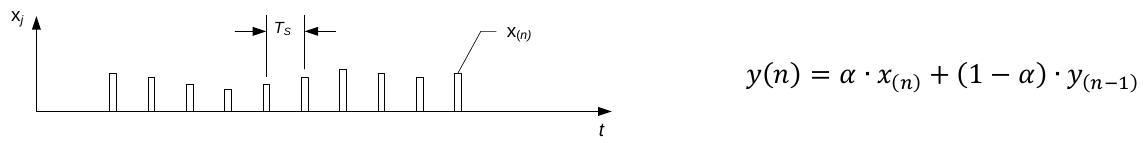
\includegraphics[width=0.95\textwidth]{../img/filter_2a.png} \\
    The advantage of the exponential filter is the ability to adjust the level of noise reduction by changing the smoothing coefficient $\alpha$ $(0 < \alpha < 1)$. The smaller the $\alpha$ , the greater the noise reduction, but the slower the filter responds to changes in the input signal.
    
    \item Assess the correctness of the filter's operation using the schemes shown below (Fig. 3). \\
    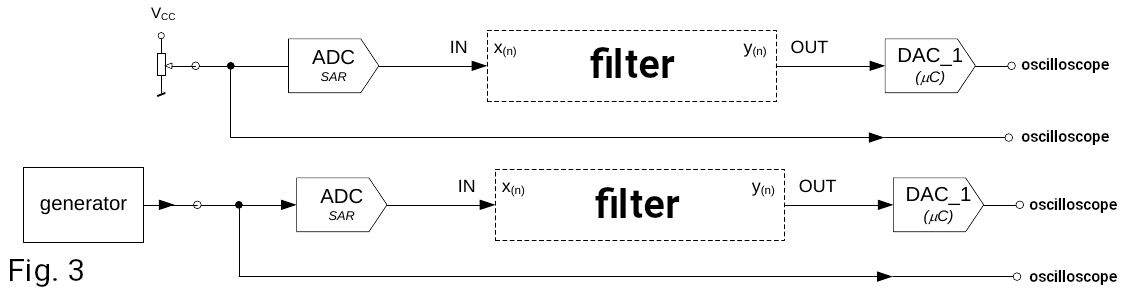
\includegraphics[width=0.95\textwidth]{../img/filter_2b.png}

    \item Investigate the filter's impulse and step response using the scheme shown below (Fig. 4). This requires writing a program to generate unit impulses and steps. \\
    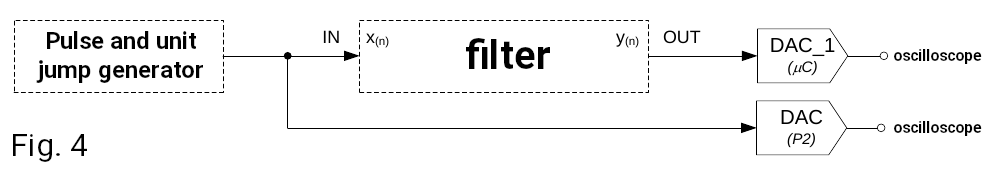
\includegraphics[width=0.95\textwidth]{../img/filter_c.png}
\end{enumerate}

\subsection*{Notes}
\begin{itemize}
    \item the samples are stored in RAM – ensure no conflict with the area occupied by the \textit{stack}
    \item suggested number of samples in the window – a power of 2
    \item for calculating the filter’s output signal, consider the possibility of exceeding the processor's word width
\end{itemize}

\subsection*{Grading}
\begin{itemize}
    \item tasks \textbf{A+B}: maximum 40 points
    \item tasks \textbf{A+B+C}: maximum 50 points
\end{itemize}

\subsection*{Suggested Literature}
R.G. Lyons, "Introduction to Digital Signal Processing," WKŁ.
\end{document}